\documentclass[tikz,border=8pt]{standalone}
\usepackage[T1]{fontenc}
\usepackage{lmodern}
\usepackage{tikz}
\usetikzlibrary{arrows.meta,calc,decorations.pathreplacing,fit,matrix,positioning}

\definecolor{cornellred}{HTML}{B31B1B}
\definecolor{ink}{HTML}{202124}
\definecolor{muted}{HTML}{667085}
\definecolor{line}{HTML}{AEB8C6}
\definecolor{paper}{HTML}{FFFFFF}
\definecolor{soft}{HTML}{F5F7FA}
\definecolor{camera}{HTML}{E8F4FF}
\definecolor{memory}{HTML}{F0F7EC}
\definecolor{compute}{HTML}{FFF3E6}
\definecolor{display}{HTML}{F7ECF3}
\definecolor{verify}{HTML}{EFEAFE}

\tikzset{
  font=\sffamily,
  flow/.style={
    -{Latex[length=2.6mm,width=1.8mm]},
    draw=muted,
    line width=0.8pt,
    rounded corners=2pt
  },
  dataflow/.style={
    flow,
    draw=cornellred
  },
  block/.style={
    rectangle,
    rounded corners=3pt,
    draw=line,
    line width=0.8pt,
    fill=paper,
    align=center,
    minimum width=28mm,
    minimum height=10mm,
    inner xsep=4pt,
    inner ysep=4pt
  },
  smallblock/.style={
    block,
    minimum width=22mm,
    minimum height=8mm,
    font=\sffamily\scriptsize
  },
  title/.style={
    font=\sffamily\bfseries\large,
    text=ink
  },
  labeltext/.style={
    font=\sffamily\scriptsize,
    text=muted,
    align=center
  },
  camera_block/.style={block, fill=camera, draw=blue!45!black},
  memory_block/.style={block, fill=memory, draw=green!45!black},
  compute_block/.style={block, fill=compute, draw=orange!65!black},
  display_block/.style={block, fill=display, draw=purple!45!black},
  verify_block/.style={block, fill=verify, draw=violet!50!black},
  groupbox/.style={
    draw=line,
    rounded corners=5pt,
    line width=0.7pt,
    fill=soft,
    inner sep=7pt
  }
}


\begin{document}
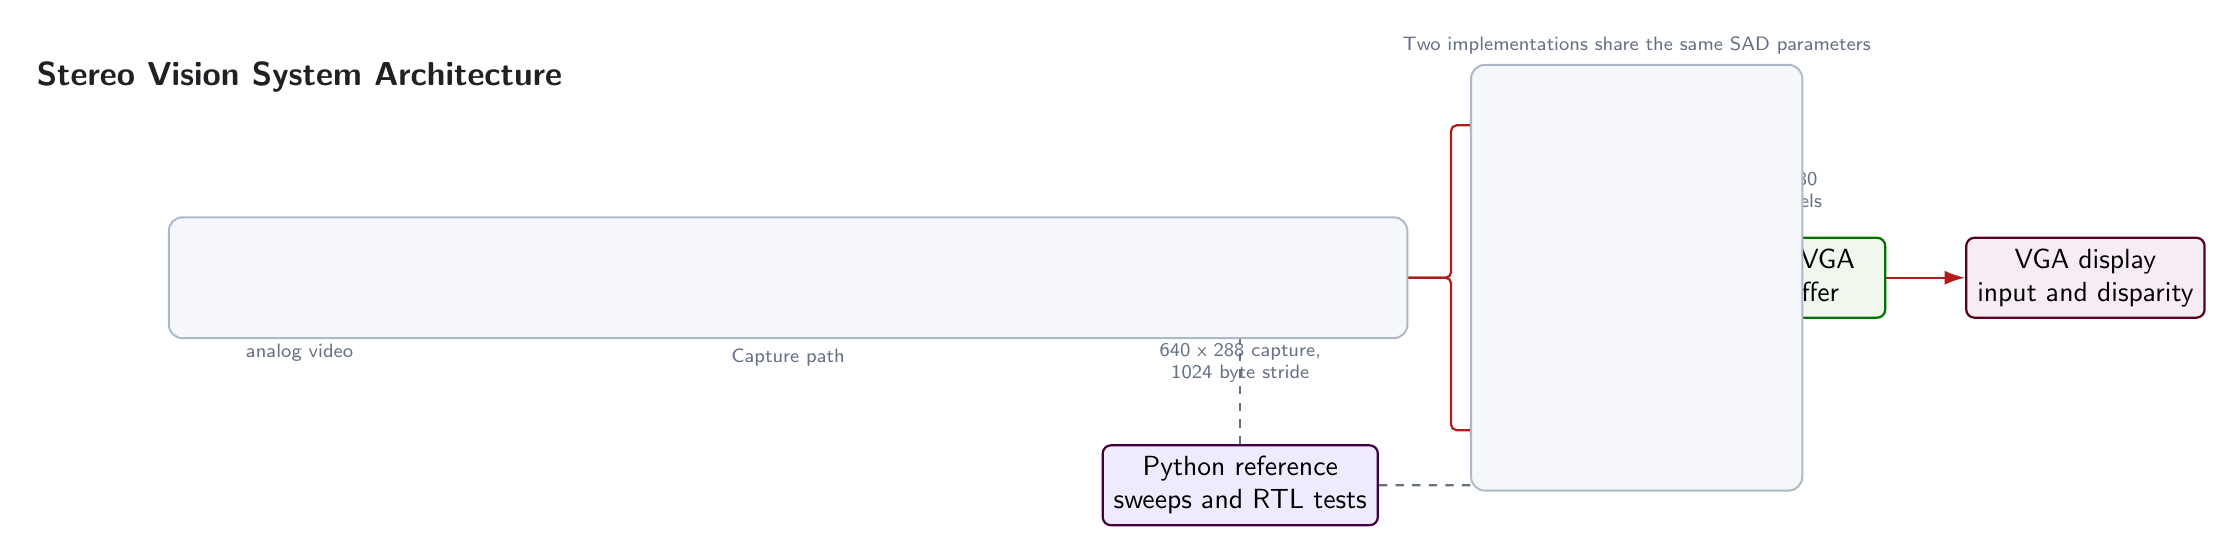
\begin{tikzpicture}[node distance=9mm and 10mm]
  \node[title] at (0, 2.55) {Stereo Vision System Architecture};

  \node[camera_block] (cams) {Dual PAL/NTSC\\cameras};
  \node[camera_block, right=of cams] (decoder) {Video front end\\and decoder};
  \node[memory_block, right=of decoder] (video_dma) {Video-In DMA\\capture stream};
  \node[memory_block, right=of video_dma] (onchip) {Custom on-chip RAM\\row-banked frame store};

  \node[compute_block, above right=9mm and 13mm of onchip] (rtl) {FPGA SAD matcher\\parallel block matching};
  \node[compute_block, below right=9mm and 13mm of onchip] (hps) {HPS C matcher\\mmap control path};
  \node[verify_block, below=16mm of onchip] (python) {Python reference\\sweeps and RTL tests};

  \node[memory_block, right=35mm of onchip] (vga_buffer) {SDRAM VGA\\pixel buffer};
  \node[display_block, right=of vga_buffer] (vga) {VGA display\\input and disparity};

  \draw[dataflow] (cams) -- (decoder);
  \draw[dataflow] (decoder) -- (video_dma);
  \draw[dataflow] (video_dma) -- (onchip);
  \draw[dataflow] (onchip.east) -- ++(8mm,0) |- (rtl.west);
  \draw[dataflow] (onchip.east) -- ++(8mm,0) |- (hps.west);
  \draw[dataflow] (rtl.east) -| (vga_buffer.north);
  \draw[dataflow] (hps.east) -| (vga_buffer.south);
  \draw[dataflow] (vga_buffer) -- (vga);

  \draw[flow, dashed] (python.north) -- (onchip.south);
  \draw[flow, dashed] (python.east) -| (rtl.south);

  \node[labeltext, below=2mm of cams] {analog video};
  \node[labeltext, below=2mm of onchip] {640 x 288 capture,\\1024 byte stride};
  \node[labeltext, above=2mm of vga_buffer] {640 x 480\\8-bit pixels};

  \node[groupbox, fit=(cams)(decoder)(video_dma)(onchip), label={[labeltext]below:Capture path}] {};
  \node[groupbox, fit=(rtl)(hps), label={[labeltext]above:Two implementations share the same SAD parameters}] {};
\end{tikzpicture}
\end{document}

